\subsection{Sous-mission X2}

	\begin{vwcol}[widths={0.65,0.2}, rule=0pt]
	\begin{minipage}{0.7\textwidth}
	\paragraph{Objectifs de la mission}

	Vérifier que ce qui apparaît sur l'image est bien de la végétation. L'image fournie est très perturbée par un bruit. Nous devons alors améliorer la visibilité en réduisant ce bruit.
	\end{minipage}

	\begin{minipage}{0.25\textwidth}
	\begin{flushright}
	\paragraph{Technique utilisée}
	
	Filtre médian
	\end{flushright}
	\end{minipage}

	\end{vwcol} 

	\begin{figure}[h]
	\centering
		\begin{multicols}{2}
		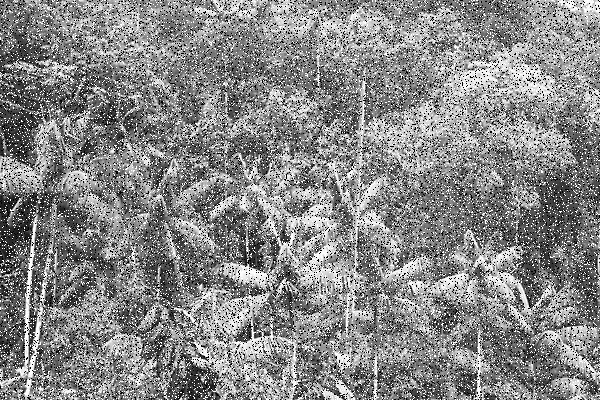
\includegraphics[scale=0.45]{images/Gliese_581d-V2.png}
		Avant

		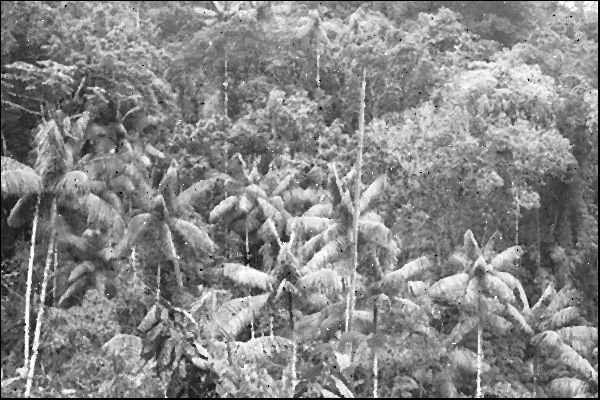
\includegraphics[scale=0.45]{images/MissionX2v2.png}
		Après
		\end{multicols}
	\end{figure}
	\vspace{-0.9cm}

	\paragraph{Procédé}
	
		Afin d'accomplir cette mission, il nous fallait nettoyer le bruit de l'image. Il était possible d'utiliser le \emph{filtre moyenneur} ou le \emph{filtre gaussien}, mais le filtre médian surpasse ces deux filtres en terme de suppression de bruit et de qualité. Le \emph{filtre médian}, permet de remplacer la valeur du pixel par la valeur médiane de son voisinage. On obtient alors une image nette mais avec un bruit réduit.